\documentclass[11pt, a4paper]{article}
\usepackage[a4paper, margin=2.0cm]{geometry}
\usepackage{xcolor}
\usepackage{titlesec}
\usepackage{hyperref}
\usepackage[T1]{fontenc}
\usepackage{mathpazo}

% new packages
\usepackage[normalem]{ulem}
\usepackage{enumitem}
\usepackage{amsmath}
\usepackage{graphicx}

% packages added for the mid submission (tables, sub-figures, pipeline diagram)
\usepackage{amssymb}
\usepackage{booktabs,array}
\usepackage[font=small,labelfont=bf]{caption}
\usepackage{subcaption}
\usepackage{float}
\usepackage{tikz}
\usetikzlibrary{arrows.meta,positioning,fit,backgrounds}
\usepackage[capitalise,nameinlink]{cleveref}
\usepackage{microtype}
\setlength{\emergencystretch}{1.5em}

\definecolor{darkblue}{RGB}{0, 32, 96}

\titleformat{\section}
  {\normalfont\Large\bfseries\color{darkblue}}{\thesection}{1em}{}
\titleformat{\subsection}
  {\normalfont\large\bfseries\color{darkblue}}{\thesubsection}{1em}{}

% Hyperlink configuration
\hypersetup{
    colorlinks=true,
    linkcolor=darkblue,
    citecolor=darkblue,
    urlcolor=darkblue
}
% this is just to signify changes
\newcommand{\remove}[1]{\sout{#1}}
\newcommand{\ankit}[1]{\textcolor{purple}{#1}}
\newcommand{\red}[1]{\textcolor{red}{#1}}
\newcommand{\green}[1]{\textcolor[rgb]{0,0.6,0}{#1}}
\newcommand{\blue}[1]{\textcolor{blue}{#1}}
\newcommand{\mauve}[1]{\textcolor[rgb]{0.58,0,0.82}{#1}}
\newcommand{\darkblue}[1]{\textcolor[rgb]{0,0,0.5}{#1}}

%to do notes
\newcommand{\todobox}[3]{%
	\colorbox{#1}{\textcolor{white}{\sffamily\bfseries\scriptsize #2}}%
	~\textcolor{blue}{#3} %
	\textcolor{#1}{$\triangleleft$}%
}
\newcommand{\todo}[1]{\todobox{red}{TODO}{#1}}

% figure colours (same as scripts/make_figures.py) and notation
\definecolor{ours}{HTML}{2a78d6}
\definecolor{inkmuted}{HTML}{52514e}
\newcommand{\R}{\mathbb{R}}
\newcommand{\SE}{\mathrm{SE}(3)}
\newcommand{\T}{\mathbf{T}}
\newcommand{\ci}{\mathbf{c}}
\newcommand{\G}{\mathcal{G}}

\title{
  \large\textnormal{CS7.503: Mobile Robotics --- Mid Submission}\\[0.5em]
  \LARGE\textbf{\color{darkblue}Lifelong Mapping \& 3D Change Detection}
}
\author{
  Ch Shreyash \\ 2024121008
  \and
  Farzana S \\ 2024121006
  \and
  Prajas Wadekar \\ 2024121009
}

\date{\small Code: \url{https://github.com/PrajasW/LM-3DCD-SG}}

\begin{document}

\maketitle

\begin{abstract}
  \noindent A robot that returns to a room with a map from an earlier visit has to find its pose in that map with no
  initial guess, decide which objects stayed, moved, appeared or disappeared, and edit the map accordingly. We pose this
  as joint relocalization and change detection on object-level 3D scene graphs, and propose a training-free pipeline
  built on one observation: objects that did not move keep their mutual distances, so the largest mutually consistent
  set of object matches is the static set and gives the pose, while smaller consistent sets are objects that moved
  together. This report covers Phase~1: scene graphs from 3RScan/3DSSG annotations, Steps~1--3 (candidate matches,
  maximum consistent set, pose), and a two-visit evaluation against four baselines in which the new visit is moved by
  an unknown rigid transform. On a 17-pair validation subset our method relocalizes 82.4\% of the pairs at the RIO
  threshold (20\,cm, 20$^\circ$) in 0.13\,s per pair and is unaffected by the transform. The learned scene-graph
  aligners SGAligner and SG-PGM drop to 35\% and 18\% (from 71--76\% and 65\% on pre-aligned frames), and dense
  FPFH+RANSAC reaches 94\% at 37$\times$ our runtime.
\end{abstract}

%======================================================================================================================
\section{Problem Statement}\label{sec:problem}

\paragraph{Motivation.} Robots in homes, offices and labs return to the same rooms many times, and the rooms change in
between. On return, the robot must relocalize in its old map although some landmarks have moved, tell moved, added and
removed objects apart from objects that are only hidden or out of view, and update the map. Replacing the old map with
the new scan deletes everything that is not currently visible, loses object identities and moves the map frame;
appending every scan keeps outdated copies and makes the map grow with every visit. Object-level 3D scene
graphs~\cite{rosinol2021kimera,wald2020learning} allow per-object edits, but, as \cref{sec:related} shows, no existing
method relocalizes without an initial guess, labels per-object changes and edits a persistent map without training.

\paragraph{Map and observations.} The map is an object-level scene graph $\G^{M}=(\mathcal{V}^M,\mathcal{E}^M)$ in a
fixed map frame. Each object node $o\in\mathcal{V}^M$ stores its points $P_o\subset\R^3$, centroid $\ci_o$, extents
$\mathbf{e}_o\in\R^3$, class $\ell_o$, height above the floor $h_o$ and change history; structural nodes hold the floor and
walls; edges carry support and spatial relations. A visit produces a point cloud split into segments, from which we build
$\G^{N}=(\mathcal{V}^N,\mathcal{E}^N)$ in the robot's own frame, related to the map frame by an unknown
$\T^{\star}\in\SE$. There is no initial guess and no odometry between visits.

\paragraph{Problem.} Given $\G^M$, $\G^N$ and the visit's depth images, estimate
\begin{enumerate}[label=(P\arabic*), leftmargin=*, itemsep=1pt, topsep=2pt]
  \item the pose $\hat\T\in\SE$ such that $\hat\T\,\ci_{o'}\approx\ci_o$ for every unchanged pair $(o,o')$, or report
        failure ($\bot$) when the observation does not determine it;
  \item a partition of the objects into \emph{static} matches $S\subset\mathcal{V}^M\times\mathcal{V}^N$ (one-to-one),
        \emph{moved} groups $\{(M_k,\T_k)\}$ with their rigid motions, \emph{removed} $R\subset\mathcal{V}^M$,
        \emph{added} $A\subset\mathcal{V}^N$ and \emph{not observed} $U\subset\mathcal{V}^M$, where $R$ and $A$ require
        depth evidence of free space and every other unexplained object goes to $U$;
  \item the updated map $\G^{M'}$, obtained by editing $\G^M$ per object so that identities persist and $|\G^{M'}|$
        grows with the number of objects, not the number of visits.
\end{enumerate}
Over visits $t=1,\dots,K$ the map is the result of applying this update repeatedly.

\paragraph{Phase-1 sub-problem and metrics.} With segments from the 3RScan/3DSSG annotations, solve (P1) and the static
part of (P2): return $(\hat\T,S)$ or $\bot$. A pair is relocalized if the rotation error
$\angle(\hat{\mathbf R},\mathbf R^\star)\le\tau_r$ and the translation error $\|\hat{\mathbf t}-\mathbf
t^\star\|\le\tau_t$, with the RIO thresholds $(\tau_t,\tau_r)\in\{(10\,\mathrm{cm},10^\circ),(20\,\mathrm{cm},20^\circ)\}$~\cite{wald2019rio};
$\bot$ counts as a failure. We also report registration recall (RMSE of the visit's points $<0.2$\,m, the criterion
of~\cite{sarkar2023sgaligner,xie2024sgpgm,liu2025sgreg}) and runtime.

\paragraph{Refinements over the proposal.} (i)~Declining ($\bot$) is part of the output and counted as a failure, so a
method cannot gain by guessing. (ii)~Descriptors must be pose invariant by construction (\cref{sec:steps}).
(iii)~Registration recall is added so that our numbers are comparable with the scene-graph alignment literature.
(iv)~Every method, learned or not, sees the same randomly transformed visits.

%======================================================================================================================
\section{Literature Review}\label{sec:related}

\paragraph{3D scene graphs.} Armeni~et~al.~\cite{armeni2019scenegraph} introduced layered 3D scene graphs.
Kimera~\cite{rosinol2021kimera} and Hydra~\cite{hughes2022hydra} build them online from SLAM, with objects assumed static
and only agents moving. 3DSSG~\cite{wald2020learning} annotates every 3RScan scan with an object-level graph (534 classes,
41 relations) and learns to predict it; SceneGraphFusion~\cite{wu2021scenegraphfusion} predicts graphs incrementally from
RGB-D, and ConceptGraphs~\cite{gu2024conceptgraphs} attaches open-vocabulary features to object nodes. Their update rules
either assume a static world or delete objects that are not re-detected, whether or not they were in view. We reuse the
representation but make the per-visit edit explicit and evidence based.

\paragraph{Scene-graph alignment and relocalization.} RIO~\cite{wald2019rio} introduced 3RScan and object instance
relocalization across rescans; X-View~\cite{gawel2018xview} localizes with semantic graphs built from views.
SGAligner~\cite{sarkar2023sgaligner} learns multi-modal node embeddings (points, relations, attributes), matches the top-$K$
nodes and registers the matched objects with GeoTransformer~\cite{qin2022geotransformer} and
GC-RANSAC~\cite{barath2018gcransac}. SG-PGM~\cite{xie2024sgpgm} casts alignment as partial graph matching, fuses
point-level features into the nodes, and re-scores point correspondences with node matches. SG-Reg~\cite{liu2025sgreg}
targets generalization and efficiency with a lighter network and a robust back-end;
SGAligner++~\cite{singh2025sgalignerpp} adds language features, and OpenSGA~\cite{chen2026opensga} moves to open-world graphs. All of these are trained, are
evaluated on sub-scans cut from the same scan, and ignore unmatched objects, so they do not output changes.
ROMAN~\cite{peterson2025roman} aligns open-set object maps for global localization with CLIPPER~\cite{lusk2021clipper};
it is the closest training-free relative of our Step~2.

\paragraph{Consistency-based data association and robust registration.} Joint compatibility~\cite{neira2001jcbb} and
PCM~\cite{mangelson2018pcm} select the largest set of mutually consistent measurements (PCM through a maximum clique, for
loop closures between maps); CLIPPER~\cite{lusk2021clipper} relaxes this to a weighted dense subgraph;
TEASER~\cite{yang2021teaser} and maximal-clique registration~\cite{zhang2023maxclique} apply the pairwise-invariant test to
point correspondences. Classical global registration pairs FPFH features~\cite{rusu2009fpfh} with
RANSAC~\cite{fischler1981ransac} and refines with ICP~\cite{besl1992icp,chen1992pointplane}. We lift the pairwise test
from points to objects, which shrinks the problem from thousands of correspondences to tens and makes the consistent sets
meaningful: the static set versus objects moved together.

\paragraph{Change detection and long-term mapping.} Objects Can Move~\cite{adam2022objects} detects moved, added and
removed parts between two \emph{aligned} scans by geometric-transformation consistency and outputs unlabelled clusters.
Living Scenes~\cite{zhu2024livingscenes} relocalizes and reconstructs objects across 3RScan rescans, again given the scan
alignment. DSG~\cite{dsg2026dynamic} labels objects stable, appeared or missing with Gaussian renderings and a language
model, uses ground-truth poses and has no ``moved'' state; 3D VSG~\cite{looper2023vsg} predicts how likely an object is to
change but does not verify it. Panoptic Multi-TSDFs~\cite{schmid2022panoptic} and Khronos~\cite{schmid2024khronos} keep
object-level volumetric maps consistent in changing scenes within one SLAM session, and LT-mapper~\cite{kim2022ltmapper}
does LiDAR lifelong mapping with change detection after alignment.

\paragraph{Viability and motivation.} \Cref{tab:capabilities} summarizes the gap: no method jointly relocalizes without
an initial guess, labels per-object changes with free-space evidence, and edits a persistent map over many visits
without training. The pieces are known to work separately: maximum-clique selection is robust to over 95\% outliers at the
point level~\cite{yang2021teaser,zhang2023maxclique}, 3RScan provides instance IDs shared across rescans together with
the moved/removed annotations needed for evaluation~\cite{wald2019rio}, and \cref{sec:experiments} shows that the
object-level version already relocalizes as well as FPFH+TEASER++ at a fraction of the cost.

\begin{table}[t]
\centering\small
\caption{Capabilities of related systems ($\checkmark$ yes, -- no, $\circ$ partial). ``Pose'' = relocalization
without an initial alignment; ``Changes'' = per-object moved/added/removed; ``Multi'' = evaluated over $>2$ visits.}
\label{tab:capabilities}
\setlength{\tabcolsep}{4pt}
\begin{tabular}{@{}lccccc@{}}
\toprule
Method & Pose & Changes & Map edit & Training-free & Multi \\
\midrule
Kimera / Hydra~\cite{rosinol2021kimera,hughes2022hydra}, ConceptGraphs~\cite{gu2024conceptgraphs} & -- & -- & $\circ$ & $\checkmark$ & -- \\
SGAligner~\cite{sarkar2023sgaligner}, SG-PGM~\cite{xie2024sgpgm}, SG-Reg~\cite{liu2025sgreg} & $\checkmark$ & -- & -- & -- & -- \\
ROMAN~\cite{peterson2025roman} & $\checkmark$ & -- & -- & $\checkmark$ & -- \\
Objects Can Move~\cite{adam2022objects} / Living Scenes~\cite{zhu2024livingscenes} & -- & $\circ$ & -- & $\checkmark$ / -- & -- \\
DSG~\cite{dsg2026dynamic} & -- & $\circ$ (no moved) & $\checkmark$ & $\circ$ (LLM) & -- \\
3D VSG~\cite{looper2023vsg} & -- & predicted only & -- & -- & -- \\
\textbf{Ours (proposed)} & $\checkmark$ & $\checkmark$ & $\checkmark$ & $\checkmark$ & $\checkmark$ \\
\bottomrule
\end{tabular}
\end{table}

%======================================================================================================================
\section{Progress So Far}\label{sec:progress}

\paragraph{Summary.} All Phase-1 deliverables of the proposal are complete:
\begin{itemize}[leftmargin=*, nosep, topsep=1pt]
  \item \textbf{Data and graphs:} loaders for 3RScan (instance PLY, labels, rescan transforms, moved/removed
        annotations) and 3DSSG; object-level scene graphs with pose-invariant node descriptors.
  \item \textbf{Steps 1--3:} candidate matching, maximum consistent set and pose with an explicit decline
        (\texttt{lifelong/}, $\sim$600 lines of Python, unit-tested on synthetic rooms).
  \item \textbf{Evaluation:} the two-visit protocol, our method, and four baselines (SGAligner, SG-PGM, FPFH+RANSAC,
        FPFH+TEASER++) run on identical inputs, with metrics, per-pair logs and all figures generated by scripts.
\end{itemize}

\begin{figure}[t]
\centering
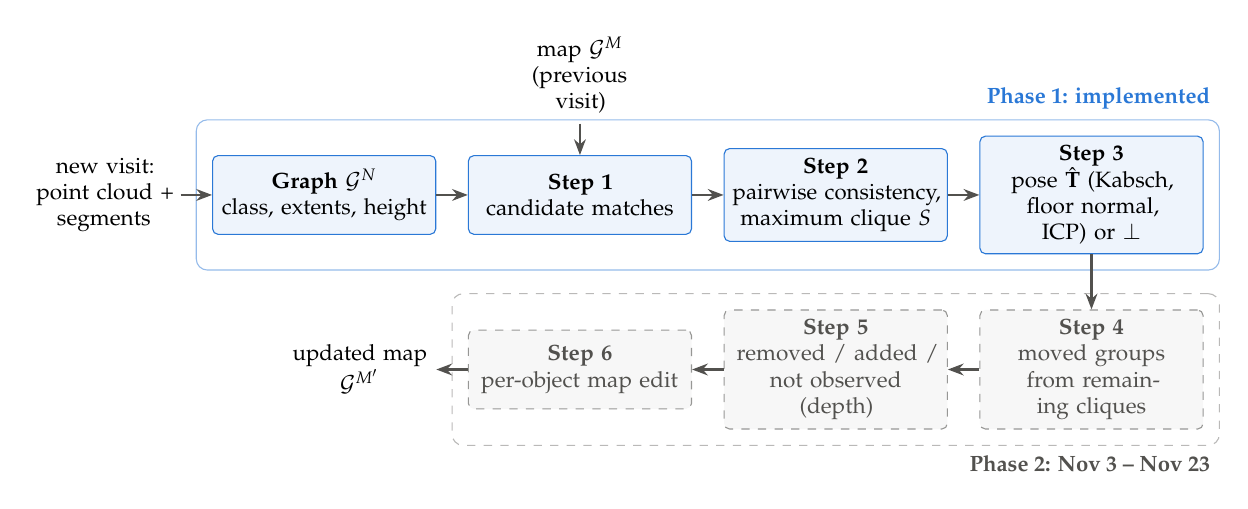
\begin{tikzpicture}[
  font=\footnotesize, node distance=3mm and 4mm,
  box/.style={draw=ours, fill=ours!8, rounded corners=2pt, align=center, minimum height=10mm, text width=26mm},
  todo/.style={draw=inkmuted!60, dashed, fill=black!3, rounded corners=2pt, align=center, minimum height=10mm,
               text width=26mm, text=inkmuted},
  io/.style={align=center, text width=17mm},
  arr/.style={-{Stealth[length=2mm]}, thick, inkmuted}]
\node[io] (scan) {new visit:\\point cloud +\\segments};
\node[box, right=of scan] (seg) {\textbf{Graph} $\G^N$\\class, extents, height};
\node[box, right=of seg] (s1) {\textbf{Step 1}\\candidate matches};
\node[box, right=of s1] (s2) {\textbf{Step 2}\\pairwise consistency,\\maximum clique $S$};
\node[box, right=of s2] (s3) {\textbf{Step 3}\\pose $\hat\T$ (Kabsch,\\floor normal, ICP) or $\bot$};
\node[io, above=4mm of s1] (map) {map $\G^M$\\(previous visit)};
\node[todo, below=7mm of s3] (s4) {\textbf{Step 4}\\moved groups\\from remaining cliques};
\node[todo, left=of s4] (s5) {\textbf{Step 5}\\removed / added /\\not observed (depth)};
\node[todo, left=of s5] (s6) {\textbf{Step 6}\\per-object map edit};
\node[io, left=of s6] (upd) {updated map\\$\G^{M'}$};
\draw[arr] (scan) -- (seg); \draw[arr] (seg) -- (s1); \draw[arr] (s1) -- (s2); \draw[arr] (s2) -- (s3);
\draw[arr] (map) -- (s1);
\draw[arr] (s3) -- (s4); \draw[arr] (s4) -- (s5); \draw[arr] (s5) -- (s6); \draw[arr] (s6) -- (upd);
\begin{scope}[on background layer]
\node[fit=(seg)(s1)(s2)(s3), draw=ours!50, rounded corners=4pt, inner sep=2mm] (p1) {};
\node[fit=(s4)(s5)(s6), draw=inkmuted!40, dashed, rounded corners=4pt, inner sep=2mm] (p2) {};
\end{scope}
\node[ours, font=\footnotesize\bfseries, anchor=south east] at (p1.north east) {Phase 1: implemented};
\node[inkmuted, font=\footnotesize\bfseries, anchor=north east] at (p2.south east) {Phase 2: Nov 3 -- Nov 23};
\end{tikzpicture}
\caption{Pipeline for one visit. Phase~1 (blue) builds the visit's graph and relocalizes it in the map; the static set
and the remaining consistent groups it produces are the inputs of Steps~4--6 (dashed, Phase~2).}
\label{fig:pipeline}
\end{figure}

\subsection{Scene-graph construction}
We load the annotated instance PLY, semantic labels and 3DSSG relations of each 3RScan scan. Floor, wall and ceiling
segments become structural nodes; every other segment with at least 50 points becomes an object node. A floor plane
$(\mathbf n,d)$ is fitted to the floor segment and oriented towards the scene. Extents are pose invariant: the vertical
extent along $\mathbf n$ and the two horizontal extents of the minimum-area bounding rectangle of the footprint (rotating
calipers on its convex hull; PCA axes were unstable for square footprints, which a unit test caught), all as 2--98\%
percentile ranges. Edges are 3DSSG relations plus proximity edges (gap $<0.3$\,m). \Cref{fig:graphs} shows the two graphs
of one pair.

\begin{figure}[t]
\centering
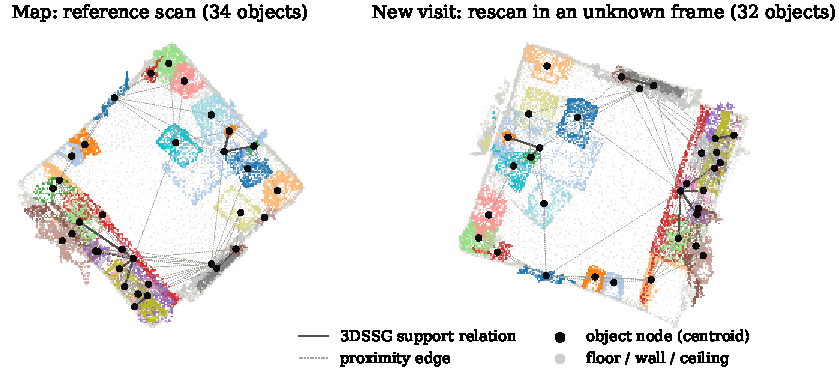
\includegraphics[width=0.7\linewidth]{figures/scene_graphs.pdf}
\caption{Scene graphs built from the annotated segments of a 3RScan reference scan (left) and one rescan (right),
top-down in each scan's own floor frame. Colours mark instances (IDs shared across scans). The rescan is in an unknown
frame; 3RScan annotates 11 of its objects as moved and one as removed. Edges: 3DSSG support relations and proximity.}
\label{fig:graphs}
\end{figure}

\subsection{Steps 1--3: relocalization}\label{sec:steps}
\paragraph{Step 1: candidate matches.} For a map object $a$ and a visit object $b$ of the same class,
\begin{equation}
  \kappa(a,b)=\sum_{k=1}^{3}\bigl|\log(e_{a,k}+\epsilon)-\log(e_{b,k}+\epsilon)\bigr|+\frac{|h_a-h_b|}{\sigma_h},
  \qquad \epsilon=5\,\mathrm{cm},\ \sigma_h=0.3\,\mathrm{m},
\end{equation}
and $\kappa=\infty$ across classes. Each map object keeps its $k=3$ cheapest visit objects and vice versa (if
$\kappa\le2.5$). Nothing depends on the robot's pose; identical objects receive several candidates and Step~2 picks among them.

\paragraph{Step 2: largest consistent set.} Two candidates $m=(a,b)$ and $m'=(a',b')$ are compatible if they are
one-to-one ($a\ne a'$, $b\ne b'$) and
\begin{equation}
 \bigl|\|\ci_a-\ci_{a'}\|-\|\ci_b-\ci_{b'}\|\bigr|\le\tau_{mm'},\quad
 \bigl|(h_a-h_{a'})-(h_b-h_{b'})\bigr|\le\tau_{mm'},\quad \tau_{mm'}=\varepsilon+\beta\,(r_m+r_{m'}),
\end{equation}
with $\varepsilon=0.1$\,m for sensor and annotation noise and $\beta=0.1$ scaling with the object radii $r$, because the
centroid of a partly observed large object shifts. The height test rejects mirror solutions that preserve all distances.
The static set $S$ is the maximum clique of the compatibility graph (igraph; ties broken by summed $\kappa$). Removing the
objects of $S$ and solving again yields further cliques of size $\ge2$: candidate groups of objects that moved together,
which Step~4 will verify. On all candidate pairs of the validation subset (\cref{fig:consistency}) the test keeps 94.5\% of
pairs of correct, unchanged matches and 25.6\% of the rest; the clique removes the remainder, since a wrong match must
agree with \emph{every} member of $S$.

\paragraph{Step 3: pose.} With $|S|\ge3$ and non-collinear centroids (second singular value of the centred centroids
$\ge0.2$\,m$\cdot\sqrt{|S|}$) we solve
\begin{equation}
  \hat{\mathbf R},\hat{\mathbf t}=\arg\min_{\mathbf R,\mathbf t}\sum_{(a,b)\in S}w_{ab}\|\mathbf R\ci_b+\mathbf t-\ci_a\|^2
  +\lambda\|\mathbf R\,\mathbf n^N-\mathbf n^M\|^2,\qquad w_{ab}=\bigl(0.1+\max(r_a,r_b)\bigr)^{-1},
\end{equation}
in closed form (weighted Kabsch/Umeyama~\cite{umeyama1991} with the floor normals as an extra direction pair), then
refine with point-to-plane ICP~\cite{chen1992pointplane} on the points of $S$ and the structural nodes (5\,cm voxels,
correspondence radius $0.3\to0.1\to0.05$\,m). If $|S|<3$, the centroids are collinear, or the ICP fitness is below 0.3,
we return $\bot$. On the development rooms, accepting collinear sets (solvable with the floor normal) only added wrong
poses, because those sets were objects that moved together, so the test stays. All thresholds were chosen on 6
\emph{training} rooms (\cref{tab:params}).

\begin{figure}[t]
\centering
\begin{subfigure}[t]{0.46\linewidth}\centering
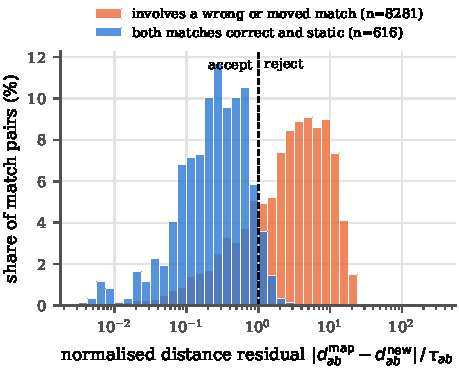
\includegraphics[width=0.92\linewidth]{figures/consistency.pdf}
\caption{Pairwise test on all candidate pairs.}\label{fig:consistency}
\end{subfigure}\hfill
\begin{subfigure}[t]{0.46\linewidth}\centering
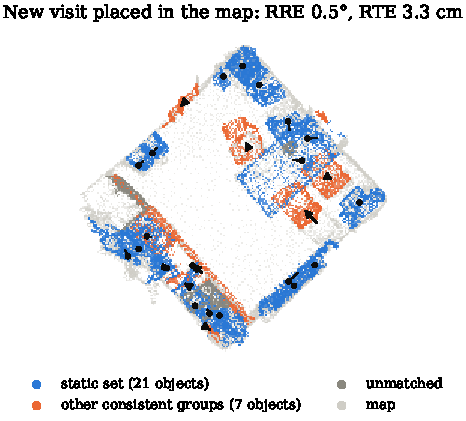
\includegraphics[width=0.72\linewidth]{figures/relocalization.pdf}
\caption{Result for the pair of \cref{fig:graphs}.}\label{fig:reloc}
\end{subfigure}
\caption{(a)~Distance residual over the tolerance $\tau_{mm'}$ for candidate pairs whose two matches are both correct and
unchanged (blue) and for all other pairs (orange), 17 validation pairs. (b)~The visit placed in the map with the
estimated pose (RTE 3.3\,cm): the static clique (blue, lines to the map centroids) gives the pose. The remaining consistent
groups (orange, arrows) are only candidates for Step~4: 4 of their 7 objects are annotated as moved; the others are static
objects missed by $S$, which Step~4 must re-test against $\hat\T$.}
\end{figure}

\subsection{Two-visit evaluation}\label{sec:experiments}
\paragraph{Data and protocol.} We use 4 validation rooms of 3RScan~\cite{wald2019rio} with 3DSSG~\cite{wald2020learning},
giving 17 pairs of a reference scan and one of its rescans (11--34 objects per map, 6--32 per visit; 81 moved, 11 removed and 3 deformed
instances in total). Each rescan is moved by a stored random transform (uniform rotation, translation
$\mathcal U(-2,2)^3$\,m) and every method receives exactly these points; $\T^\star$ comes from the 3RScan alignment and is
used only for scoring. A second run gives the rescan already aligned to the map, which is the setting in which the learned
baselines were trained and evaluated.

\paragraph{Baselines.} We chose the strongest methods with runnable 3RScan code: SG-PGM~\cite{xie2024sgpgm} and
SGAligner~\cite{sarkar2023sgaligner} with their released 3RScan-trained checkpoints (our rooms are from the validation
split, so there is no train/test leakage), and the training-free FPFH+RANSAC~\cite{rusu2009fpfh,fischler1981ransac} and
FPFH+TEASER++~\cite{yang2021teaser}, both followed by ICP. SG-Reg~\cite{liu2025sgreg} (only a ScanNet model and a C++
back-end are released) and SGAligner++~\cite{singh2025sgalignerpp} (no code) are discussed from their papers. Two fixes
were needed for a fair run (details in the appendix): SGAligner's GC-RANSAC needs score-sorted correspondences for
its PROSAC sampler (unsorted input gave no model in 53\% of aligned pairs), and FPFH normals are oriented towards the scan
centre (Open3D's default sign depends on the frame and halved TEASER++'s success under rotation).

\begin{table}[t]
\centering\small
\caption{Two-visit relocalization on 17 validation pairs with a random rigid transform. ``Ret.'' = pose returned;
succ.\ = RIO thresholds (cm/$^\circ$); RR = RMSE $<0.2$\,m; median errors over returned poses; time per pair (pose
only). Last column: succ.\ 20/20 when the rescan is pre-aligned (the baselines' own setting).}
\label{tab:results}
\setlength{\tabcolsep}{3.2pt}
\begin{tabular}{@{}lcccccccc@{}}
\toprule
Method & Ret.\,\% & 10/10 & 20/20 & RR & RRE ($^\circ$) & RTE (cm) & Time (s) & Aligned \\
\midrule
SGAligner~\cite{sarkar2023sgaligner} & 47.1 & 35.3 & 35.3 & 35.3 & 1.24 & 4.7 & 2.73 & 70.6--76.5 \\
SG-PGM~\cite{xie2024sgpgm} & 100 & 17.6 & 17.6 & 17.6 & 80.2 & 145 & 2.99 & 64.7 \\
FPFH + TEASER++~\cite{yang2021teaser} & 100 & 70.6 & 82.4 & 82.4 & 1.07 & 3.2 & 1.69 & 82.4 \\
FPFH + RANSAC~\cite{rusu2009fpfh} & 100 & \textbf{76.5} & \textbf{94.1} & \textbf{94.1} & 1.07 & \textbf{3.2} & 4.82 & 88.2 \\
\midrule
Ours, centroid pose only & 94.1 & 52.9 & 76.5 & 82.4 & 1.55 & 7.6 & $<$0.01 & 82.4 \\
\textbf{Ours (Steps 1--3)} & 94.1 & 70.6 & 82.4 & 82.4 & \textbf{0.99} & 3.3 & \textbf{0.13} & 82.4 \\
\bottomrule
\end{tabular}
\end{table}

\begin{figure}[t]
\centering
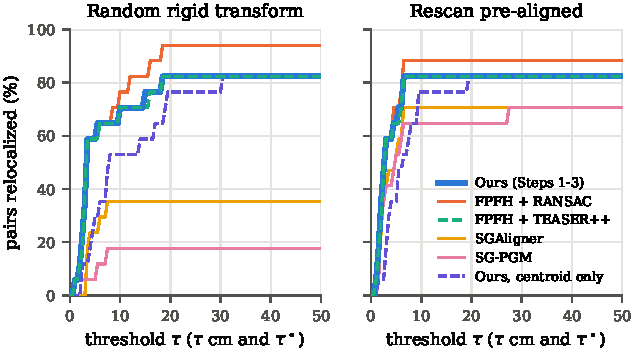
\includegraphics[width=0.58\linewidth]{figures/success_curves.pdf}\hspace{1.5em}
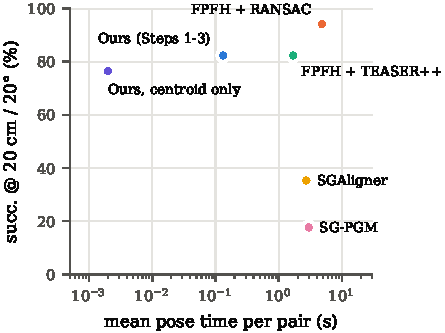
\includegraphics[width=0.3\linewidth]{figures/runtime.pdf}
\caption{Left: share of pairs relocalized as the threshold grows (translation $\tau$\,cm and rotation $\tau^\circ$
jointly), with a random transform (our protocol) and with pre-aligned frames. Ours and FPFH+TEASER++ coincide on this
subset except near 15\,cm. Right: success at 20\,cm/20$^\circ$ against mean pose time.}
\label{fig:curves}
\end{figure}

\paragraph{Results} (\cref{tab:results,fig:curves}).
(i)~\emph{Invariance.} Our scores are identical with and without the random transform. The learned aligners collapse
(SGAligner 71--76\%$\to$35\%, SG-PGM 65\%$\to$18\%): their node encoders consume object points in world coordinates,
and SG-PGM's published random-transform evaluation rotated only the registration points, not the scene-graph objects.
(ii)~\emph{Accuracy and cost.} Ours matches FPFH+TEASER++ and trails FPFH+RANSAC by two pairs at 37$\times$ lower cost:
Steps~1--2 take 1.5\,ms on 4--77 candidates and ICP takes the rest. ICP halves the error of the centroid-only pose
(7.6$\to$3.3\,cm) and raises succ.\ 10/10 from 53\% to 71\%. Unlike the point-level methods, ours also returns object
correspondences (static-set precision 60.5\%, recall 58.5\%; mostly swaps among identical objects, harmless for the pose).
(iii)~\emph{Failures} (\cref{fig:perpair}, appendix). One café room has a row of identical table--chair--menu sets:
a shift by one set is consistent for 8 objects against 7 for the truth, and without walls ICP cannot tell them apart
(RANSAC fails one of the two pairs too). One rescan sees only 6 objects and we decline. On the development rooms the
other declines are rooms where \emph{every} object moved, for which structure-only registration would still give a pose.

%======================================================================================================================
\section{Timeline for the Remainder of the Project}\label{sec:timeline}
\begin{table}[H]
\centering\small
\setlength{\tabcolsep}{4pt}
\caption{Plan for Phase~2 and the demo (weekly milestones, 2026).}\label{tab:timeline}
\begin{tabular}{@{}>{\raggedright\arraybackslash}p{2.1cm}>{\raggedright\arraybackslash}p{11.6cm}>{\raggedright\arraybackslash}p{2.3cm}@{}}
\toprule
Dates & Work package & Deliverable \\
\midrule
Oct 27--Nov 2 & Full 3RScan validation split (47 rooms, 110 rescans) for all methods; structure-only fallback (floor/wall registration) when $|S|<3$; repeated-layout check using wall evidence. & Final Phase-1 table \\
Nov 3--9 & \textbf{Step 4}: motion of each remaining clique; single-object moves by direct ICP. \textbf{Step 5}: project unmatched map objects into the visit's depth frames with $\hat\T$: free space $\Rightarrow$ removed, occluded or out of view $\Rightarrow$ not observed; added only over previously observed free space. & Change P/R per type \\
Nov 10--16 & \textbf{Step 6}: per-object map edit with change history and free-space record; multi-visit setting (rooms with $\ge3$ scans); map size and share of objects at the correct place per visit. & Multi-visit curves \\
Nov 17--23 & Predicted segments (Mask3D~\cite{schult2023mask3d} or SceneGraphFusion~\cite{wu2021scenegraphfusion}; class mismatch as a cost instead of a hard gate); ablations; final report. & Final report (Nov 23) \\
Nov 24--26 & Demo: relocalization, change labels and map edits on 3RScan rooms (interactive viewer and video). & Demo (Nov 26) \\
\bottomrule
\end{tabular}
\end{table}

\noindent\textbf{Risks.} Predicted segments break one-to-one matching (we will allow many-to-one candidates);
Step~5 needs the RGB-D sequences (frames will be subsampled); the subset is small, so the full split comes first.

\newpage
\bibliographystyle{plain}
\bibliography{references}

\clearpage
\appendix
\section{Appendix: Per-Pair Results and Implementation Details}
\begin{figure}[h]
\centering
\begin{minipage}{0.46\linewidth}\centering
\captionsetup{justification=raggedright,singlelinecheck=false}
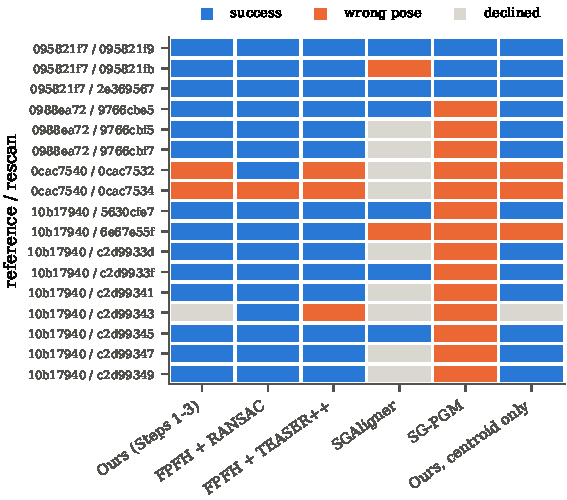
\includegraphics[width=\linewidth]{figures/per_pair.pdf}
\captionof{figure}{Per-pair outcome at 20\,cm/20$^\circ$ (random transform). Rows are grouped by reference scan.}
\label{fig:perpair}
\end{minipage}\hfill
\begin{minipage}{0.51\linewidth}\small\raggedright
\captionsetup{justification=raggedright,singlelinecheck=false}
\captionof{table}{Parameters of our method (\texttt{configs/default.yaml}), chosen on 6 training rooms (22 pairs). A
sweep over $\varepsilon$, $\beta$, $k$ and the cost gate gave 19/22 correct and no wrong poses almost everywhere.}
\label{tab:params}
\footnotesize\setlength{\tabcolsep}{3pt}
\begin{tabular}{@{}lll@{}}
\toprule
Step & Parameter & Value \\
\midrule
Graph & min.\ segment size & 50 points \\
1 & candidates per object $k$ & 3 (both directions) \\
1 & extent offset $\epsilon$, height scale $\sigma_h$ & 5\,cm, 0.3\,m \\
1 & cost gate & $\kappa\le2.5$, same class \\
2 & tolerance $\varepsilon$, $\beta$ & 0.10\,m, 0.10 \\
2 & moved-group min.\ size & 2 \\
3 & min.\ static objects / spread & 3 / 0.2\,m \\
3 & ICP voxel, radii & 5\,cm; 0.3, 0.1, 0.05\,m \\
3 & min.\ ICP fitness & 0.3 \\
\bottomrule
\end{tabular}\\[0.8em]
\textbf{Baseline setup.} Our adapter exports the pairs to SGAligner's data layout and runs its own preprocessing;
SG-PGM reads the same files. One conda environment (PyTorch 2.7.1/CUDA~12.8, RTX~2080\,Ti) runs SGAligner ($K=2$ node
matches, 3DMatch GeoTransformer, GC-RANSAC) and SG-PGM (released weights, GeoTransformer backbone). SGAligner's own
preprocessing builds the per-scan pickles from the exported full scans (attribute vocabulary 164, relations 41, as in
the checkpoints); 3DSSG ``inside'' relations are dropped because that preprocessing rejects them. SG-PGM's internal
augmentation is disabled since the transform is already in the data. Source commits, patches and package versions are
in the repository (\texttt{baselines/}).\\[0.5em]
\textbf{Data and models.} Scans come from the Hugging Face mirror
\href{https://huggingface.co/datasets/maartenImjalli143/3RScan}{\texttt{maartenImjalli143/3RScan}}; metadata and 3DSSG
from the official release. No models were trained, so there are no Hugging Face or WandB model artefacts.\\[0.5em]
\textbf{Reproduction.} \texttt{bash scripts/run\_all.sh} runs the tests, pair generation, all methods and the
evaluation; \texttt{scripts/make\_figures.py} regenerates every figure from \texttt{results/}.
\end{minipage}
\end{figure}

\end{document}
